%!TEX root = ../main.tex



\section{sommario}

\begin{itemize}
  

    \item \textbf{ML Engineering Process Perspective (Discover-Play-Develop-Deploy, DevOps/MLOps)} (slides 27--28)
    \item \textbf{AI Product/Service Landscape \& Risk Spectrum} (slides 29--32)
    \begin{itemize}
        \item AI product/service heterogeneity across industries (slides 29--30)
        \item The AI systems spectrum: risk and autonomy (slide 31)
        \item AI-centric vs System-centric perspectives (slide 32)
    \end{itemize}
    \item \textbf{AI-Centric vs System-Centric Examples} (slides 33--36)
    \begin{itemize}
        \item LLM-based agents architecture (slide 34)
        \item ADS/ADAS system-centric example (slide 35)
        \item Technical requirements for the hands-on pipeline (slide 36)
    \end{itemize}
    \item \textbf{Full Pipeline Example -- Setup \& Requirements} (slides 37--39)
    \begin{itemize}
        \item Environment setup instructions (conda, git clone) (slide 37)
        \item Managing stakeholder requirements with Jira (slides 38--39)
    \end{itemize}
    \item \textbf{Full Pipeline Example -- Exploratory Analysis ("Play")} (slides 40--41)
    \begin{itemize}
        \item Data prep for Prophet forecasting model (slide 40)
        \item Ad hoc plotting code and its limitations (slide 41)
    \end{itemize}
    \item \textbf{Full Pipeline Example -- Development Process Selection} (Agile vs Waterfall) (slide 42)
    \item \textbf{Full Pipeline Example -- Code Version Control} (slides 43--47)
    \begin{itemize}
        \item Git branching example (slide 43)
        \item Merge conflicts (slide 44)
        \item Git workflow: main/dev/feature/release/hotfix branches (slide 45)
        \item Git flow diagram (slide 46)
        \item Pull requests and code review (slide 47)
    \end{itemize}
    \item \textbf{Full Pipeline Example -- Model Version Control (MLflow)} (slides 48--52)
    \begin{itemize}
        \item MLflow installation and imports (slide 48)
        \item Prophet model wrapper class (slide 49)
        \item Logging parameters, metrics, and models (slide 50)
        \item MLflow tracking UI setup (slide 51)
        \item MLflow UI screenshot (slide 52)
    \end{itemize}
    \item \textbf{Full Pipeline Example -- Deployment Infrastructure Options} (slides 53--55)
    \begin{itemize}
        \item On-premise deployment (slide 53)
        \item Infrastructure-as-a-Service (IaaS) (slide 54)
        \item Platform-as-a-Service (PaaS) (slide 55)
    \end{itemize}
    \item \textbf{Full Pipeline Example -- CI/CD \& DevOps/MLOps Lifecycle Tables} (slides 56--59)
    \begin{itemize}
        \item CI/CD concept overview (slide 56)
        \item Dev lifecycle activities: testing, linting, formatting, building (slide 57)
        \item ML lifecycle activities: training, predicting, staging, monitoring (slide 58)
        \item Ops lifecycle activities: releasing, deploying, monitoring (slide 59)
    \end{itemize}
    \item \textbf{Full Pipeline Example -- CI/CD Automation with GitHub Actions} (slides 60--61)
    \begin{itemize}
        \item Workflow definition YAML (slide 60)
        \item Dependency installation, linting, and testing steps (slide 61)
    \end{itemize}
    \item \textbf{Full Pipeline Example -- Continuous Model Performance Testing} (slides 62--63)
    \begin{itemize}
        \item Test fixtures: dataset and model loading (slide 62)
        \item Model inference and performance assertions (slide 63)
    \end{itemize}
    \item \textbf{Summary / Conclusion} (slide 64)
\end{itemize}

\pagebreak

\section{Introduction to AI Systems Engineering}



This lecture, delivered by Prof. Roberto Pietrantuono, opens the core part of the course: \textbf{AI Systems Engineering}. The goal of the course segment is to move from a purely algorithmic view of AI (i.e., "how do I train a model?") to a \emph{systems engineering} view: how do we design, build, integrate, verify, deploy, and maintain an AI-based system as a whole, considering data, computing infrastructure, human factors, and responsible AI concerns together.

\begin{defbox}{AI Systems Engineering}
The discipline that applies classical systems engineering principles (requirements elicitation, architecture design, integration, verification and validation, lifecycle management) to systems whose core functional building block is one or more AI/ML components. It treats the AI model not as an isolated artifact, but as one subsystem embedded in a larger technical, organizational, and human ecosystem.
\end{defbox}

\subsection{Outline}

The lecture is structured around five macro-blocks, which will be treated in strict order because each one logically depends on the previous:

\begin{itemize}
    \item The \textbf{Functional Architecture} -- answers the question "\emph{What} does an AI system consist of?" It is a conceptual decomposition into functional blocks (sensors, data conditioning, ML, human-machine teaming, computing, responsible AI), independent of any specific technology.
    \vspace{0.2cm}
    \item \textbf{From What to How: The Implementation Framework} -- once we know \emph{what} the building blocks are, we need a framework describing \emph{how} to realize them in practice (technology choices, processes, people/organization).
    \vspace{0.2cm}
    \item \textbf{Development Process} -- the concrete methodology (e.g., Agile/CRISP-DM-like cycles: Discover, Play, Develop, Deploy) used to go from a business problem to a working AI solution.
    \vspace{0.2cm}
    \item \textbf{DevOps, MLOps} -- the operational practices and tooling (CI/CD, versioning, monitoring) that make the development process repeatable, automated, and production-grade.
    \vspace{0.2cm}
    \item \textbf{A first simple full production pipeline} -- a hands-on, end-to-end example that ties all the previous concepts together on a toy project.
\end{itemize}

This is essentially a top-down narrative: \emph{architecture} (what) $\rightarrow$ \emph{framework} (how, at a high level) $\rightarrow$ \emph{process} (how, methodologically) $\rightarrow$ \emph{operations} (how, technically/automatically) $\rightarrow$ \emph{example} (how, concretely).

\subsubsection*{ How to Build an AI System?}

This is a transition/section-divider slide posing the central question of the lecture: \emph{how do we systematically build an AI system}, rather than simply training a model in isolation? This framing already hints at the key idea developed later: building a model that performs well on a benchmark is only a small part of building an AI \emph{system} that is deployed, monitored, maintained, and trusted in the real world.

\subsubsection{ The System Engineering High-Level V-Model}

The V-Model is a classical systems/software engineering lifecycle model, here applied to AI systems. It is drawn as two diagonal lines forming a "V": the left branch represents \emph{decomposition} (from abstract requirements down to concrete lower-level elements), and the right branch represents \emph{integration and verification} (building back up from realized lower-level elements to the validated overall system).

\begin{defbox}{V-Model}
A systems engineering lifecycle representation in which:
\begin{itemize}
    \item  the left descending branch decomposes a system into progressively more detailed sub-elements (via architecture decomposition and definition, guided by integration/verification/validation planning).
    \item the right ascending branch mirrors each decomposition step with a corresponding integration and verification step, culminating in a fully realized and validated system/solution.
\end{itemize}
\end{defbox}



Below is a simplified TikZ rendition of the V-Model as shown in the slide:
% Nel preambolo, assicurati di avere:
% \usetikzlibrary{arrows.meta}

% Nel preambolo, assicurati di avere:
% \usetikzlibrary{arrows.meta}

\begin{center}
\resizebox{\textwidth}{!}{%
\begin{tikzpicture}[
    every node/.style={font=\small, align=center},
    box/.style={draw, rounded corners, fill=blue!8, minimum width=2.8cm, minimum height=0.8cm, inner sep=3pt}
]
    % ---------- LEFT DESCENDING BRANCH ----------
    \node[box] (req)      at (0,5)   {Stakeholder's\\requirements};
    \node[box] (sysdev)   at (1.3,4) {System\\development};
    \node[box] (upperdev) at (2.6,3) {Upper-level system\\element development};
    \node[box] (lowerdev) at (3.9,2) {Lower-level system\\element development};

    % ---------- BOTTOM OF THE V ----------
    \node[box, fill=orange!15, draw=orange!70!black] (real) at (5.5,0.7) {Lower-level system\\element realization};

    % ---------- RIGHT ASCENDING BRANCH ----------
    \node[box] (upperreal) at (7.1,2) {Upper-level system\\element realization};
    \node[box] (sysreal)   at (8.4,3) {System\\realization};
    \node[box, fill=green!15, draw=green!50!black] (solution) at (9.7,4) {Solution};

    % ---------- ARROWS ----------
    \draw[-{Latex[length=2mm]}, thick] (req) -- (sysdev);
    \draw[-{Latex[length=2mm]}, thick] (sysdev) -- (upperdev);
    \draw[-{Latex[length=2mm]}, thick] (upperdev) -- (lowerdev);
    \draw[-{Latex[length=2mm]}, thick] (lowerdev) -- (real);
    \draw[-{Latex[length=2mm]}, thick] (real) -- (upperreal);
    \draw[-{Latex[length=2mm]}, thick] (upperreal) -- (sysreal);
    \draw[-{Latex[length=2mm]}, thick] (sysreal) -- (solution);

    % ---------- TOP LABELS ----------
    \node[font=\bfseries\itshape, align=center] at (1.8,6.2) {Architecture decomposition\\and definition};
    \node[font=\bfseries\itshape, align=center] at (7.9,6.2) {Architecture Integration\\and Verification};

\end{tikzpicture}%
}
\end{center}



Reading the model as presented in the figure:

\begin{itemize}
    \item \textbf{Left (descending) branch -- decomposition}:
    \begin{itemize}
        \item \emph{Stakeholder's requirements} -- the starting point: what do the users/business actually need?
        \item \emph{System development} -- requirements are translated into a system-level design.
        \item \emph{Upper-level system element development} -- the system is broken into major sub-elements.
        \item \emph{Lower-level system element development} -- each upper-level element is further decomposed into finer-grained elements, down to the point where they can actually be built/realized.
    \end{itemize}
    \vspace{0.2cm}
    \item \textbf{Bottom of the V}: \emph{Lower-level system element realization} -- the actual construction/implementation of the smallest elements (e.g., writing the code for a specific module, training a specific model component).
    \vspace{0.4cm}
    \item \textbf{Right (ascending) branch -- integration and verification}:
    \begin{itemize}
        \item \emph{Upper-level system element realization} -- lower-level elements are integrated back into upper-level elements, and each integration step is verified.
        \item \emph{System realization} $\rightarrow$ \emph{Solution} -- the fully integrated system is verified and validated against the original stakeholder requirements, producing the final solution.
    \end{itemize}
\end{itemize}



\textbf{Why this matters for AI systems.} In a classical software system, the "lower-level elements" are modules and functions. In an AI system, they also include \emph{data pipelines}, \emph{trained models}, and \emph{human-machine interaction logic} -- each of which needs its own decomposition, realization, and verification strategy, which is exactly what the "Functional Architecture" introduced in the next slides will formalize.

\subsubsection{A Functional AI System Architecture}

This slide introduces the notion of a \textbf{Functional AI System Architecture}, i.e., the answer to \emph{"What"} an AI system is made of, independently of the specific technologies chosen to implement it. This is the conceptual "parts list" of any AI system, regardless of domain (healthcare, automotive, finance, etc.).

\begin{defbox}{Functional Architecture}
A technology-agnostic decomposition of a system into functional blocks -- each performing a well-defined role and connected to the others via well-defined information flows -- that specifies \emph{what} the system must do, as opposed to an implementation architecture, which specifies \emph{how} (with which technologies/tools) it is realized.
\end{defbox}

The distinction between \emph{functional} (What) and \emph{implementation} (How) architecture is a recurring theme of the whole lecture (it reappears explicitly in the outline item "From What to How"), and mirrors the classical systems-engineering separation between \emph{logical architecture} and \emph{physical architecture}.

\subsubsection*{The "WHAT": The Functional AI System Architecture}

This is the key reference diagram of the lecture (adapted from Martinez \& Kifle, \emph{Artificial Intelligence: A Systems Approach from Architecture Principles to Deployment}, 2024).

\vspace{0.3cm}


\begin{center}
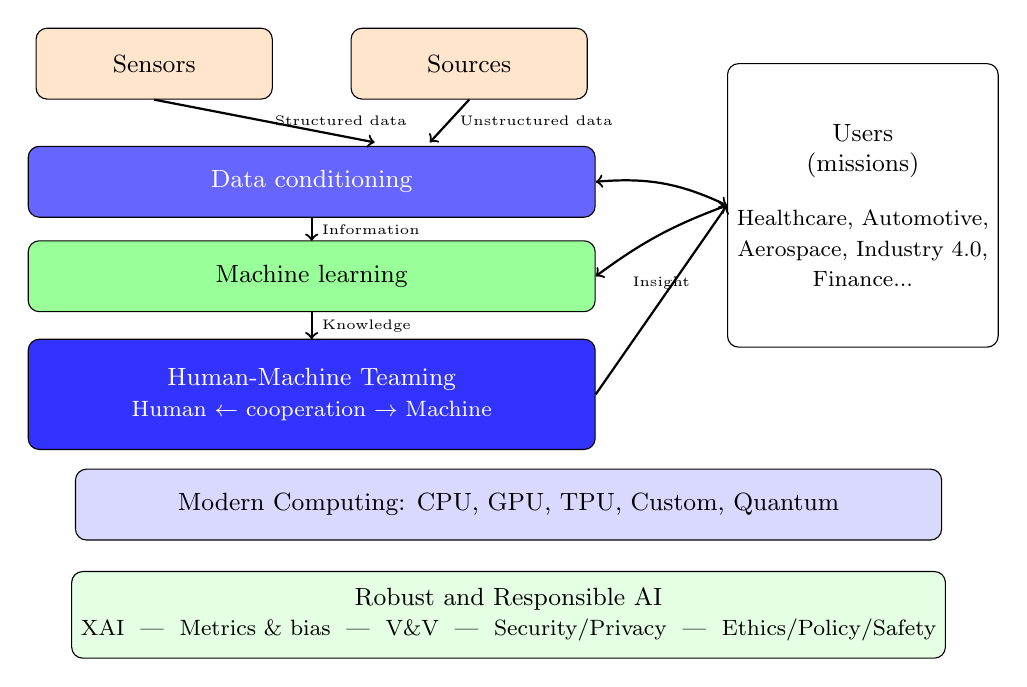
\begin{tikzpicture}[
    every node/.style={font=\small, align=center},
    box/.style={draw, rounded corners, minimum height=0.9cm},
    node distance=0.4cm
]
    % Top row: Sensors / Sources / Users
    \node[box, fill=orange!20, minimum width=3cm] (sensors) at (0,6) {Sensors};
    \node[box, fill=orange!20, minimum width=3cm] (sources) at (4,6) {Sources};
    \node[box, minimum width=3cm, minimum height=3.6cm] (users) at (9,4.2) {Users\\(missions)\\[0.3cm] \footnotesize Healthcare, Automotive,\\ \footnotesize Aerospace, Industry 4.0,\\ \footnotesize Finance...};

    % Data conditioning
    \node[box, fill=blue!60, text=white, minimum width=7.2cm] (dc) at (2,4.5) {Data conditioning};

    % Machine learning
    \node[box, fill=green!40, minimum width=7.2cm] (ml) at (2,3.3) {Machine learning};

    % HMT
    \node[box, fill=blue!80, text=white, minimum width=7.2cm, minimum height=1.4cm] (hmt) at (2,1.8) {Human-Machine Teaming\\ \footnotesize Human $\leftarrow$ cooperation $\rightarrow$ Machine};

    % Computing layer
    \node[box, fill=blue!15, minimum width=11cm] (comp) at (4.5,0.4) {Modern Computing: CPU, GPU, TPU, Custom, Quantum};

    % Responsible AI layer
    \node[box, fill=green!10, minimum width=11cm, minimum height=1.1cm] (rai) at (4.5,-1) {Robust and Responsible AI\\ \footnotesize XAI\ \ |\ \ Metrics \& bias\ \ |\ \ V\&V\ \ |\ \ Security/Privacy\ \ |\ \ Ethics/Policy/Safety};

    % Arrows
    \draw[->, thick] (sensors.south) -- (2.8,5) node[midway, right, font=\tiny] {Structured data};
    \draw[->, thick] (sources.south) -- (3.5,5) node[midway, right, font=\tiny] {Unstructured data};
    \draw[->, thick] (dc.south) -- (2,3.75) node[midway, right, font=\tiny] {Information};
    \draw[->, thick] (ml.south) -- (2,2.5) node[midway, right, font=\tiny] {Knowledge};
    \draw[->, thick] (hmt.east) -- (users.west) node[midway, above, font=\tiny] {Insight};

    % Bidirectional feedback arrows to users
    \draw[<->, thick] (dc.east) to[bend left=15] (users.west);
    \draw[<->, thick] (ml.east) to[bend left=8] (users.west);
\end{tikzpicture}
\end{center}



It lays out the functional blocks of \emph{any} AI system and how information flows through them, from raw data acquisition to insight delivery to end users, all resting on a computing layer and cross-cut by a "Robust and Responsible AI" layer.

\begin{defbox}{Functional AI System Architecture (the six layers)}
\begin{enumerate}
    \item \textbf{Sensors \& Sources} -- acquisition of \emph{structured} data (sensors: e.g., radar, cameras, IoT) and \emph{unstructured} data (sources: e.g., social media, documents, open data).
    \item \textbf{Data Conditioning} -- transforms raw structured/unstructured data into \emph{Information}: cleaning, storage, integration, quality assessment.
    \item \textbf{Machine Learning} -- transforms Information into \emph{Knowledge} via (un)supervised learning, reinforcement learning, or other paradigms.
    \item \textbf{Human-Machine Teaming} -- transforms Knowledge into actionable \emph{Insight}, on a spectrum ranging from fully human-driven, through human-machine cooperation, to fully autonomous machine action.
    \item \textbf{Modern Computing} -- the horizontal infrastructure layer (CPU, GPU, TPU, custom accelerators, quantum) that powers every layer above it.
    \item \textbf{Robust and Responsible AI} -- a cross-cutting layer (Explainable AI, metrics/bias assessment, V\&V against standards/benchmarks, security/privacy, policy/ethics/safety/training) that must be considered at \emph{every} stage, not only at the end.
\end{enumerate}
\end{defbox}

\textbf{Reading the data-flow (bottom-up on the functional stack):}

\begin{itemize}
    \item \emph{Sensors} produce \textbf{structured data} (e.g., a GPS reading, a table of measurements); \emph{Sources} produce \textbf{unstructured data} (e.g., text, images, social posts).
    \vspace{0.2cm}
    \item Both flow into \textbf{Data Conditioning}, which turns raw data into \textbf{Information} (cleaned, integrated, contextualized data ready for analysis).
    \vspace{0.2cm}
    \item Information flows into \textbf{Machine Learning}, which applies (un)supervised learning, reinforcement learning, or other techniques to turn Information into \textbf{Knowledge} (patterns, predictive models, learned representations).
    \vspace{0.2cm}
    \item Knowledge flows into \textbf{Human-Machine Teaming}, which turns it into \textbf{Insight} -- something directly actionable/useful for the end user.
\end{itemize}

\textbf{The Human-Machine Teaming spectrum.} This block is drawn with a gradient bar from \emph{Human} to \emph{Machine}, passing through \emph{Human-Machine cooperation}. This encodes the idea that "insight delivery" is not binary (either fully manual or fully automated): different AI systems sit at different points of this autonomy spectrum, and the right point depends on the risk, criticality, and regulatory context of the application (a theme that will be developed later in the course as the "AI Systems Spectrum").

\begin{defbox}{Human-Machine Teaming (HMT)}
The functional block responsible for converting the knowledge produced by machine learning into insight that supports (or drives) a decision, at a level of human involvement that ranges continuously from full human control, through cooperative human-machine decision-making, to full machine autonomy.
\end{defbox}

\textbf{Bidirectional arrows.} Note that the arrows connecting Data Conditioning, Machine Learning, and Human-Machine Teaming to the \emph{Users (missions)} box on the right are drawn as \emph{bidirectional}. This is intentional: it is not a purely feed-forward pipeline. Users (and their missions -- e.g., surgery, autonomous driving, drone operation, Industry 4.0, financial monitoring, as depicted in the icons) can inject feedback, corrections, or new requirements back into any layer (e.g., a human operator relabeling data, or providing feedback that triggers retraining). This closes the loop and is a first hint at why AI systems require \emph{continuous} lifecycle management (MLOps), rather than a one-shot build.

\textbf{The two horizontal foundation layers.}

\begin{itemize}
    \item \textbf{Modern Computing}: CPU, GPU, TPU, Custom (e.g., ASICs, FPGAs), and Quantum computing. This layer underlies \emph{every} functional block above it -- data conditioning, ML training/inference, and even human-machine interfaces all consume computing resources, and the choice of hardware has direct implications on cost, latency, and scalability (a topic that reappears in the "Implementation Framework" discussed later).
    \vspace{0.2cm}
    \item \textbf{Robust and Responsible AI}: this layer is drawn beneath everything else but conceptually applies \emph{across} all layers (it is a cross-cutting concern, not a final step). It comprises five pillars:
    \begin{itemize}
        \item \emph{Explainable AI (XAI)} -- techniques to make model decisions interpretable.
        \item \emph{Metrics and bias assessment} -- quantitative evaluation of fairness and performance.
        \item \emph{V\&V (standards \& benchmarks)} -- verification and validation against recognized standards and benchmark datasets.
        \item \emph{Security, Privacy} -- protection from adversarial attacks and data leakage.
        \item \emph{Policy, ethics, Safety and training} -- organizational/regulatory/ethical governance (this is where frameworks such as the EU AI Act, mentioned later in the course, become relevant).
    \end{itemize}
\end{itemize}



\textbf{Take-away.} This diagram is the reference mental model for the rest of the course: whenever a new topic is introduced (e.g., data storage strategies, ML paradigms, DevOps/MLOps pipelines), it should be mentally located within one of these six layers, which helps understand \emph{why} that topic matters and how it connects to the rest of the system.

\subsection{ Managing Big Data: The 4 "Vs"}

This chapter introduces the classical framework used to characterize the complexity of a Big Data problem \emph{before} deciding on storage, processing, or ML strategy. The four axes are not independent metrics with fixed values -- they are \emph{sliders}: each real-world dataset sits somewhere between the two extremes shown for each "V", and the position on each slider drives different engineering trade-offs.

\begin{defbox}{The 4 Vs of Big Data}
\begin{itemize}
    \item \textbf{Volume} -- the scale of the data (Few entities $\rightarrow$ Many entities). Drives the choice between vertical and horizontal scaling.
    \vspace{0.2cm}
    \item \textbf{Velocity} -- the required collection/processing latency (Short $\rightarrow$ Long). Drives the choice between batch and streaming architectures.
    \vspace{0.2cm}
    \item \textbf{Variety} -- the diversity of data representation/input (Single $\rightarrow$ Many types; structured vs. unstructured). Drives the choice between relational (SQL) and schema-flexible (NoSQL) storage.
    \vspace{0.2cm}
    \item \textbf{Veracity} -- the reliability/provenance of the data (Trusted $\rightarrow$ Untrusted). Drives the need for data quality checks, validation, and lineage tracking.
\end{itemize}

\end{defbox}

Each "V" also correlates with an \emph{increasing-difficulty} dimension: higher Volume $\Rightarrow$ harder to manage relationships and dimensionality; higher Velocity $\Rightarrow$ tighter response-time requirements; lower Veracity $\Rightarrow$ worse signal-to-noise ratio.



\textbf{Why this matters.} Every subsequent design decision in the "Data Conditioning" layer (storage engine, SQL vs. NoSQL, batch vs. streaming, edge vs. cloud) is a direct consequence of where the problem sits on these four sliders. This chapter is therefore the conceptual entry point for the rest of the Data Conditioning block.

\subsubsection{Data Conditioning: Key Questions}

This chapter is a checklist of the questions an AI systems engineer should ask \emph{before} committing to a specific data architecture. It operationalizes the 4 Vs into concrete engineering decisions.

\begin{center}
\begin{tabular}{p{5.5cm}p{7.5cm}}
\toprule
\textbf{Question} & \textbf{Comment} \\
\midrule
What insight does the customer need? & Work backward from the expected result to the needed data (goal-driven design, not data-driven). \\[0.2cm]
What data input is required to achieve the desired insight? & Make sure the data are \emph{curated} (i.e., quality-checked and relevant), not just abundant. \\[0.2cm]
Are the incoming data and required processing batched or streaming? & Field-deployed applications typically combine both: streaming inference at the edge, batch training/analytics in the cloud. \\[0.2cm]
Can we solve the problem with ML techniques other than Deep Learning? & Deep learning is powerful only when data are statistically representative of the population/scenarios; simpler models may suffice otherwise. \\[0.2cm]
Do we need edge computing? & Relevant when operating under low-capacity or intermittent network links. \\[0.2cm]
How do we protect the AI system from adversarial AI (e.g., data poisoning)? & AI systems are fragile and easy to fool; security must be considered from the data layer up. \\
\bottomrule
\end{tabular}
\end{center}

\begin{defbox}{Data Poisoning}
An adversarial attack in which an attacker injects maliciously crafted samples into the training data, causing the model to learn incorrect patterns or to embed a hidden backdoor triggered by specific inputs at inference time.
\end{defbox}



\subsubsection{Data Storage Solutions}

This chapter surveys how data storage technology has evolved to cope with the 4 Vs, moving beyond the classical relational model.

\begin{defbox}{OLTP (Online Transaction Processing)}
A class of database workloads/systems designed for many small, fast, atomic read/write transactions over a fixed schema (e.g., a banking system recording a purchase). The relational model was originally designed for OLTP.
\end{defbox}

Key points from the slide:

\begin{itemize}
    \item \textbf{Beyond the relational model}: as data volume/variety grew, database types proliferated beyond OLTP-oriented relational systems.
    \vspace{0.2cm}
    \item \textbf{Distributed storage \& data locality}: the surviving architectural principle is to \emph{move the computation to the data} (rather than moving large data to a central computation node), reducing network I/O.
    \vspace{0.2cm}
    \item \textbf{Hadoop} (HDFS for storage + MapReduce for processing + YARN for cluster scheduling) was the historical de-facto standard for distributed big-data processing; it is now largely considered legacy technology.
    \vspace{0.2cm}
    \item \textbf{Modern approach}: object storage (S3-like) combined with open \emph{table formats} (Delta Lake, Apache Iceberg, Apache Hudi) that \emph{decouple storage from compute} -- i.e., the data sits in cheap object storage while multiple independent compute engines can query it.
    \vspace{0.2cm}
    \item \textbf{Layer separation -- storage, transport, processing are distinct}:
    \begin{itemize}
        \item \emph{Transport}: Kafka -- a durable, replayable, append-only log for moving data between systems.
        \item \emph{Processing}: Spark (batch \& micro-batch), Flink (true record-at-a-time streaming), Ray (distributed Python/ML workloads).
    \end{itemize}
    \vspace{0.2cm}
    \item \textbf{NoSQL clarification}: NoSQL does not mean "unstructured" -- it means \emph{schema-on-read} (the schema is interpreted by the application when reading, not enforced by the database engine when writing). Four families exist: key-value, document, wide-column, graph. NoSQL trades \emph{joins} and \emph{multi-row transactions} for \emph{horizontal scalability}.
    \vspace{0.2cm}
    \item \textbf{Edge computing constraints}: at the edge (IoT), the binding constraints are \emph{memory}, \emph{energy}, and \emph{intermittent connectivity} -- not raw throughput, which is usually the bottleneck in cloud-scale systems.
\end{itemize}

\subsubsection{Storage Trade-offs: Consistency, Latency, Planes}

This chapter covers the fundamental theoretical trade-offs that govern distributed data storage design.

\begin{defbox}{CAP Theorem}
In a distributed data store, during a network \textbf{P}artition, a system cannot simultaneously guarantee both \textbf{C}onsistency (every read receives the most recent write) and \textbf{A}vailability (every request receives a non-error response). A system must therefore be designed as either \emph{CP} (favoring consistency) or \emph{AP} (favoring availability) when a partition occurs.
\end{defbox}

\begin{defbox}{PACELC Theorem}
An extension of CAP that is more practically relevant to system design: \emph{if there is a Partition (P)}, choose between \emph{Availability (A)} and \emph{Consistency (C)} (this is the CAP trade-off); \emph{Else (E)}, i.e., during normal operation with no partition, choose between \emph{Latency (L)} and \emph{Consistency (C)}. The "Else" branch is the trade-off that is paid almost continuously, since network partitions are comparatively rare events.
\end{defbox}

\begin{defbox}{OLTP vs. OLAP Planes}
\begin{itemize}
    \item \textbf{OLTP (Operational plane)}: row-oriented, optimized for low-latency point access; serves the live application.
    \item \textbf{OLAP (Analytical plane)}: column-oriented, optimized for large scans; serves training and reporting workloads.
\end{itemize}
\end{defbox}

\textbf{Critical ML-specific consequence:} the offline (OLAP, training) and online (OLTP, serving) planes \emph{must agree} on the same feature definition. If a feature is computed slightly differently at training time than at serving time, the model experiences \textbf{training/serving skew} -- a silent and dangerous failure mode where the model's production performance degrades even though offline evaluation looked fine.

\begin{defbox}{Training/Serving Skew}
A discrepancy between the feature values (or their computation logic) used during model training and those used during online inference, causing the deployed model to receive inputs statistically different from what it was trained on, and consequently to underperform in production despite good offline metrics.
\end{defbox}

\subsubsection{SQL and NoSQL Comparison}

This chapter provides a systematic point-by-point comparison between the two historical database paradigms.

\begin{center}
\begin{tabular}{p{5.7cm}p{7.3cm}}
\toprule
\textbf{SQL} & \textbf{NoSQL} \\
\midrule
Relational database, fixed columns/rows; typically structured data. & Non-relational, flexible schema (schema-on-read); mostly semi-structured data. Four families: key-value, document, wide-column, graph. \\[0.15cm]
Follows a specific schema (e.g., last name, first name, address, phone as fixed columns). & Structured data is stored, but nested inside a single aggregate rather than as row-column pairs; the schema is enforced by the \emph{application}, not the engine. \\[0.15cm]
ACID is native: multi-row transactions, referential integrity, declarative joins. & Historically \emph{BASE} (Basically Available, Soft State, Eventually Consistent) rather than ACID; joins/referential integrity are pushed to the application layer. \\[0.15cm]
Scales vertically by default; horizontal scale requires sharding, which breaks joins/cross-shard transactions. & Horizontal scale is the design goal: partitioning and replication are built in. \\[0.15cm]
Originated early 1970s, driven by transactional processing needs. & Originated mid-2000s, driven by rapid-ingestion needs (e.g., internet search). \\
\bottomrule
\end{tabular}
\end{center}

\begin{defbox}{ACID vs. BASE}
\begin{itemize}
    \item \textbf{ACID}: Atomicity, Consistency, Isolation, Durability -- the classical transactional guarantee of relational databases.
    \item \textbf{BASE}: Basically Available, Soft state, Eventually consistent -- a weaker but more scalable consistency model historically favored by NoSQL systems.
\end{itemize}
\end{defbox}

\textbf{Important caveat}: this SQL/NoSQL dichotomy is \emph{dated}. Many modern NoSQL engines now offer ACID transactions (e.g., MongoDB multi-document transactions since v4.0, DynamoDB transactions), while distributed SQL systems (Google Spanner, CockroachDB, TiDB) provide horizontal scalability \emph{together with} SQL semantics and ACID guarantees. The table should be read as describing two \emph{historical design centers}, not two mutually exclusive technology categories one must choose between today.

\subsubsection{NoSQL Database Types}

This chapter details the four (plus one hybrid) families of NoSQL databases previously mentioned .

\begin{defbox}{The NoSQL Families}
\begin{itemize}
    \item \textbf{Key-value databases} -- the simplest NoSQL model: a key maps directly to an opaque value/attribute set (e.g., Customer \#ID $\rightarrow$ Attributes). \emph{Example: Amazon DynamoDB.}
    \vspace{0.2cm}
    \item \textbf{Key-value cache} -- like key-value stores, but data is held in RAM for very low latency access. \emph{Examples: Redis, Memcached, Apache Ignite.}
    \vspace{0.2cm}
    \item \textbf{Document databases} -- the key is a document ID; the value is a hierarchical tree structure (JSON, XML, YAML) containing the whole document. \emph{Example: MongoDB.}
    \vspace{0.2cm}
    \item \textbf{Wide-column databases} -- each "column family" behaves like a container of rows in a relational table, but the set of columns can differ from row to row. \emph{Examples: Google Bigtable, Cassandra.}
    \vspace{0.2cm}
    \item \textbf{Graph databases} -- data is stored as nodes (entities, e.g., people) connected by edges (relationships, e.g., social connections). \emph{Example: Neo4J.}
\end{itemize}
\end{defbox}

 This taxonomy is the concrete technological realization of the "Variety" axis from the 4 Vs: the more heterogeneous the data representation, the more likely a specialized NoSQL family (rather than a single relational schema) is the right storage fit.

\subsubsection{Stores the Generic Taxonomy Misses}

This slide highlights two increasingly important storage categories that do \emph{not} fit neatly into the classical SQL/NoSQL taxonomy, both of which are central to modern ML systems (especially LLM/RAG applications and production ML pipelines).

\begin{defbox}{Vector Store}
A specialized storage/index engine designed to hold high-dimensional embedding vectors and to perform \emph{approximate nearest-neighbour (ANN) search} over them -- used for retrieval, Retrieval-Augmented Generation (RAG), deduplication, and near-duplicate detection. It is \emph{approximate by construction}: recall is deliberately traded off for lower latency and memory usage. \emph{Dedicated engines: Milvus, Qdrant, Weaviate, FAISS (as a library); or an index inside an existing DB: pgvector, Elasticsearch, OpenSearch.}
\end{defbox}

\textbf{Critical operational caveat:} changing the embedding model invalidates the entire vector index (the new embeddings are not comparable to the old ones). This creates both a \emph{re-embedding cost} (all data must be re-encoded) and a \emph{versioning problem}: the index version and the embedding-model version must be pinned together, or silent retrieval quality degradation will occur.

\begin{defbox}{Feature Store}
A system that stores a \emph{single feature definition} but serves it through two different paths:
\begin{itemize}
    \item An \textbf{offline store} -- historical, point-in-time correct data used for \emph{training}.
    \item An \textbf{online store} -- low-latency key-value lookup used for \emph{serving} (inference).
\end{itemize}

\end{defbox}

\emph{Examples: Feast, Tecton, or various cloud-managed feature stores.}



\subsubsection{Example: Key-Value Store}

This chapter provides a concrete worked example of how a customer's data would be modeled in a key-value store, illustrating the design principles of the key-value family introduced.

\textbf{Data model.} A single key (\texttt{CustomerID}) maps to a single, nested, opaque \emph{aggregate object} containing everything related to that customer:

\begin{center}
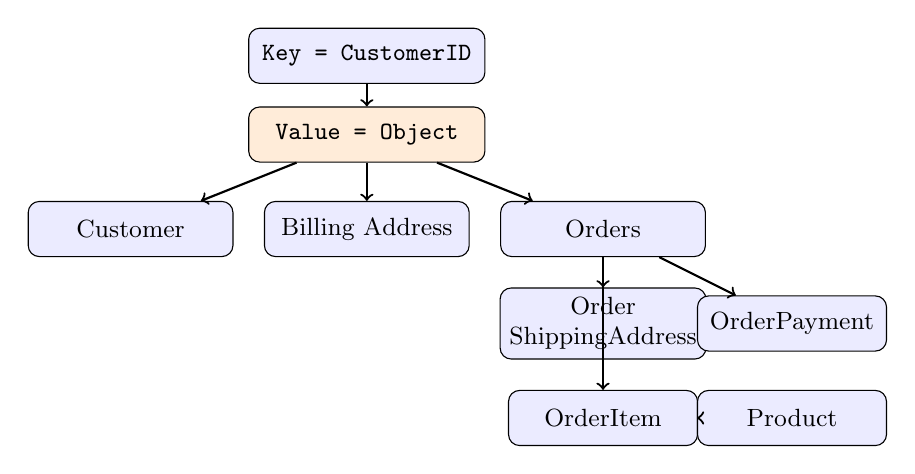
\begin{tikzpicture}[
    every node/.style={font=\small, align=center},
    box/.style={draw, rounded corners, fill=blue!8, minimum height=0.7cm}
]
    \node[box, minimum width=3cm] (key) at (0,3) {\texttt{Key = CustomerID}};
    \node[box, fill=orange!15, minimum width=3cm] (val) at (0,2) {\texttt{Value = Object}};

    \node[box, minimum width=2.6cm] (cust) at (-3,0.8) {Customer};
    \node[box, minimum width=2.6cm] (bill) at (0,0.8) {Billing Address};
    \node[box, minimum width=2.6cm] (ord) at (3,0.8) {Orders};

    \node[box, minimum width=2.4cm] (shipadd) at (3,-0.4) {Order\\ShippingAddress};
    \node[box, minimum width=2.4cm] (pay) at (5.4,-0.4) {OrderPayment};
    \node[box, minimum width=2.4cm] (item) at (3,-1.6) {OrderItem};
    \node[box, minimum width=2.4cm] (prod) at (5.4,-1.6) {Product};

    \draw[->, thick] (key) -- (val);
    \draw[->, thick] (val) -- (cust);
    \draw[->, thick] (val) -- (bill);
    \draw[->, thick] (val) -- (ord);
    \draw[->, thick] (ord) -- (shipadd);
    \draw[->, thick] (ord) -- (pay);
    \draw[->, thick] (ord) -- (item);
    \draw[->, thick] (item) -- (prod);
\end{tikzpicture}
\end{center}

\begin{defbox}{Key-Value Aggregate Model}
The entire nested structure associated with a key is treated as a single \emph{opaque blob} (aggregate) by the storage engine: it can only be retrieved or written whole, via \texttt{get} and \texttt{put} operations on the key. The engine performs no server-side querying on nested fields, no joins, and no cross-key transactions.
\end{defbox}

\textbf{What this design buys, and what it costs (as stated on the slide):}

\begin{itemize}
    \item \textbf{Cost / consequence}: since there is no server-side query on nested fields, \emph{the access pattern must be known at design time} -- you model the data around the query you intend to run, not the other way around (as you would with a flexible relational schema).
    \vspace{0.2cm}
    \item \textbf{Denormalisation is the norm}: the same underlying fact (e.g., a customer's address) may be duplicated across multiple aggregates for fast, single-key retrieval, and it becomes the \emph{application's responsibility} (not the database's) to keep these duplicated copies consistent.
\end{itemize}



\subsubsection{ Example: Wide-Column Database}

This chapter provides the example for the wide-column family introduced , showing the progressive structure from a single column up to a full column family across multiple rows.

\begin{defbox}{Wide-Column Data Model -- Building Blocks}
\begin{itemize}
    \item \textbf{Column}: a simple \texttt{name}/\texttt{value} pair.
    \item \textbf{Super Column}: a named collection of multiple \texttt{name}/\texttt{value} columns grouped under one super-column name.
    \item \textbf{Column Family}: identified by a \texttt{row key}, containing an arbitrary set of \texttt{name}/\texttt{value} pairs (columns) -- crucially, \emph{different rows in the same family can have different columns}.
    \item \textbf{Super Column Family}: a row key containing multiple named super columns, each itself containing its own set of columns.
\end{itemize}
\end{defbox}

\textbf{Concrete illustration.} Three rows (\texttt{Smith}, \texttt{John}, \texttt{Harry}), each identified by a row key, but each having a \emph{different} set of columns:

\begin{center}
\begin{tabular}{lll}
\toprule
\textbf{Row Key} & \textbf{Columns present} & \textbf{Comment} \\
\midrule
Smith & Gender, Age & has both attributes \\
John & Gender & missing Age -- no problem, no NULL needed \\
Harry & Gender, Education & has a different second attribute than Smith \\
\bottomrule
\end{tabular}
\end{center}

Each individual column value also carries its own \texttt{Timestamp}, allowing versioned/point-in-time reads -- a feature exploited by systems such as Google Bigtable and Cassandra.

\textbf{Why this matters.} This heterogeneity across rows (no rigid, uniform column set) is exactly what distinguishes a wide-column NoSQL store from a classical relational table, where every row must populate the exact same set of columns (using \texttt{NULL} for missing values). It gives wide-column stores excellent horizontal scalability and sparse-data efficiency, at the cost of the relational guarantees (joins, multi-row ACID transactions) discussed in Slide 11.

\subsubsection{Data Wrangling / Munging}

This chapter describes the standard pipeline of activities needed to transform raw data into a dataset ready for modeling -- effectively a detailed breakdown of what happens \emph{inside} the "Data Conditioning" functional block.

\begin{defbox}{Data Wrangling (Munging)}
The process of transforming raw, heterogeneous, and possibly messy data into a clean, structured, well-documented, and reproducible dataset suitable for machine learning, typically organized into the sequential stages of discovery, structuring, cleaning, preparation/enrichment, validation, and publishing.
\end{defbox}

\begin{center}
\begin{tabular}{p{3.6cm}p{9.4cm}}
\toprule
\textbf{Stage} & \textbf{Issues/Activities} \\
\midrule
Data discovery & Analyze and understand the data: are the required data available and representative? What is their provenance? Is there bias? \\[0.15cm]
Data structuring & Organize raw data into a structured form. \\[0.15cm]
Cleaning, data quality & Corrections, formatting, de-duplication, handling of missing/incomplete data, outlier detection, imputation, rescaling, re-sampling. \emph{Every choice here is a modeling assumption and must be documented} (note: over/underfitting and the bias-variance trade-off belong to the modeling stage, not to cleaning). \\[0.15cm]
Preparation, Enriching & Curse of dimensionality, dimensionality reduction, feature engineering and selection, data augmentation, labeling and label quality (inter-annotator agreement). \\[0.15cm]
Validating & Consistency, accuracy, privacy and security, bias checks. \emph{Split discipline}: use temporal or grouped splits where the i.i.d. assumption does not hold (e.g., time series, or multiple samples from the same subject). \\[0.15cm]
Publishing & Version and pin the dataset (via hash, snapshot, or table version) so results are reproducible; prepare the dataset for downstream use by users or software. \\
\bottomrule
\end{tabular}
\end{center}

\begin{defbox}{i.i.d. Assumption \& Non-i.i.d. Splits}
Many ML algorithms assume training samples are \emph{independent and identically distributed (i.i.d.)}. When this assumption is violated -- e.g., in time series data (samples are temporally correlated) or when multiple samples come from the same entity (e.g., multiple images of the same patient) -- a naive random train/test split leaks information across the split, giving an overly optimistic performance estimate. \emph{Temporal splits} (train on the past, test on the future) or \emph{grouped splits} (ensure all samples from one entity stay entirely in either train or test) must be used instead.
\end{defbox}

\subsubsection{Data Management Strategy (FAIR Principles)}

This chapter focuses specifically on the \emph{governance and policy} side of data conditioning: how data should be managed as an organizational asset, independent of the specific storage technology chosen.

\begin{defbox}{FAIR Principles}
A set of guiding principles for scientific/organizational data management, stating that data should be:
\begin{itemize}
    \item \textbf{F}indable -- easily discoverable (e.g., through metadata, naming conventions, catalogs).
    \item \textbf{A}ccessible -- retrievable by authorized users through defined tools/repositories.
    \item \textbf{I}nteroperable -- usable together with other data/tools via standard formats.
    \item \textbf{R}e-usable -- clearly licensed and documented so it can be reused in other contexts/projects.
\end{itemize}
\end{defbox}

\textbf{Key questions the strategy must answer (as listed on the slide):}

\begin{itemize}
    \item What data can be shared/disclosed, and how? What tools/repositories should be used for sharing?
    \vspace{0.2cm}
    \item What naming conventions should be adopted?
    \vspace{0.2cm}
    \item How/where should data be stored -- considering security (e.g., encryption), privacy, and reliability (e.g., fault-tolerant replicas, distributed systems)?
    \vspace{0.2cm}
    \item What (if any) data can be re-used, and under which licensing options?
    \vspace{0.2cm}
    \item How do the data need to be consumed -- streaming or batch processing (linking back to the storage/processing distinctions made in Slides 9--10)?
\end{itemize}

\textbf{Integration with earlier material.} This slide effectively closes the loop on the "Robust and Responsible AI" cross-cutting layer from the functional architecture: security and privacy concerns raised here (encryption, access control) are concrete instances of that layer applied specifically to data.

\subsubsection{ Data Governance (EU AI Act, Art. 10)}

This chapter grounds the data conditioning discussion in a concrete regulatory framework: Article 10 of the EU AI Act, which imposes legally binding data-governance obligations on \emph{high-risk} AI systems.

\begin{defbox}{EU AI Act -- Article 10 (Data Governance)}
Regulation (EU) 2024/1689. For high-risk AI systems, the training, validation, and test datasets must be subject to \emph{documented data governance}, covering:
\begin{itemize}
    \item Collection design and data origin.
    \item Preparation operations: annotation, labelling, cleaning, updating, enrichment.
    \item Explicit assumptions about what the data are meant to represent.
    \item Examination of possible biases affecting health, safety, or fundamental rights.
    \item Identification of data gaps and how they are addressed.
\end{itemize}
Per Art. 10(3), datasets must be relevant, sufficiently representative, and -- as far as possible -- error-free and complete for the intended purpose and deployment context.
\end{defbox}

\textbf{Key regulatory details from the slide:}

\begin{itemize}
    \item \textbf{Art. 10(5)}: special-category personal data (e.g., data revealing health, ethnicity) may be processed \emph{strictly for bias detection and correction}, under appropriate safeguards -- an explicit, narrow exception to normal data-protection restrictions.
    \vspace{0.2cm}
    \item \textbf{GDPR is not sufficient}: GDPR compliance (lawful basis, purpose limitation, minimisation) does \emph{not} automatically satisfy Art. 10 -- the two sets of obligations are \emph{parallel}, not substitutable. GDPR governs whether you may process personal data at all; Art. 10 governs the \emph{quality and representativeness} of the dataset used for a high-risk AI system.
    \vspace{0.2cm}
    \item \textbf{Timeline}: the \emph{Digital Omnibus on AI} (in force 27 July 2026) has deferred high-risk obligations to \textbf{2 Dec 2027} for stand-alone Annex III systems and \textbf{2 Aug 2028} for embedded Annex I systems. Note that the Art. 50 \emph{transparency} duties were \emph{not} deferred and remain on the original timeline.
\end{itemize}

\begin{defbox}{Engineering Consequence of Art. 10}
Representativeness, bias examination, and data-gap identification are not merely ethical aspirations -- they are \textbf{dataset-level test obligations} under EU law for high-risk systems. To be auditable, they require \emph{versioning}, \emph{lineage} (tracking where each data point came from and how it was transformed), and \emph{documented ownership} -- i.e., precisely the same artifacts (dataset publishing/pinning from Slide 16, FAIR documentation from Slide 17) already motivated on purely engineering grounds.
\end{defbox}

\subsection{Machine Learning by Strategy}

This chapter provides a taxonomy of Machine Learning paradigms, organized by \emph{learning strategy} -- i.e., by the type and amount of supervision available during training. This taxonomy fills in the details of the "(Un)supervised L., Reinforcement L., Others..." annotation that appeared next to the Machine Learning block in the functional architecture diagram.

\begin{defbox}{Learning Paradigm}
A classification of ML algorithms based on the nature of the training signal available: whether labeled examples are provided (supervised), only unlabeled data is available (unsupervised), a mix of both (semi-supervised), labels are derived automatically from the data itself (self-supervised), or the signal comes from a reward obtained through interaction with an environment (reinforcement learning).
\end{defbox}

\pagebreak

\textbf{Taxonomy breakdown:}

\begin{itemize}
    \item \textbf{Supervised learning} -- learns a mapping from labeled input-output pairs. Divided into:
    \begin{itemize}
        \item \emph{Classification} (discrete output): Decision Tree, SVC (Support Vector Classifier), K-NN (K-Nearest Neighbors), Neural Network.
        \item \emph{Regression} (continuous output): (Non-)Linear Regression, SVR (Support Vector Regression), Neural Networks, Regression Trees.
    \end{itemize}
    \vspace{0.2cm}
    \item \textbf{Semi-supervised learning} -- uses a small amount of labeled data together with a larger pool of unlabeled data. Divided into:
    \begin{itemize}
        \item \emph{Inductive} -- learns a general rule applicable to new, unseen data.
        \item \emph{Transductive} -- makes predictions only for the specific unlabeled instances available during training, without generalizing to a broader rule.
    \end{itemize}
    \vspace{0.2cm}
    \item \textbf{Unsupervised learning} -- no labels at all; the algorithm finds structure in the data on its own. Divided into:
    \begin{itemize}
        \item \emph{Clustering}: K-Means, Hierarchical, Probabilistic clustering.
        \item \emph{Association}: Rule mining, Itemset mining.
    \end{itemize}
    \vspace{0.2cm}
    \item \textbf{Self-supervised learning} -- labels are automatically generated from the structure of the input data itself (e.g., predicting a masked word from its context), without manual annotation.
    \vspace{0.2cm}
    \item \textbf{Reinforcement Learning (RL)} -- an agent learns by interacting with an environment and receiving reward signals. Characterized along several orthogonal axes:
    \begin{itemize}
        \item \emph{Off-policy vs. On-policy} -- whether the policy being learned is different from (off-policy) or the same as (on-policy) the policy used to generate the training data.
        \item \emph{Offline vs. Online} -- whether learning happens from a fixed, pre-collected dataset (offline) or through live interaction with the environment (online).
        \item \emph{Value-, Policy-, Model-based} -- whether the agent learns a value function, a policy directly, or a model of the environment's dynamics.
    \end{itemize}
\end{itemize}

Below is a schematic reconstruction of the taxonomy tree:

\begin{center}
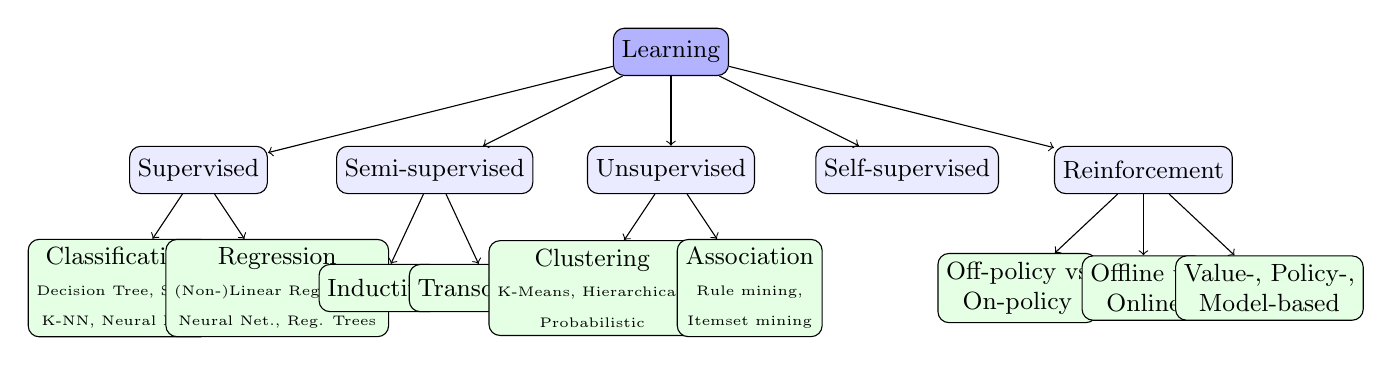
\begin{tikzpicture}[
    every node/.style={font=\small, align=center},
    box/.style={draw, rounded corners, fill=blue!8, minimum height=0.6cm, inner sep=3pt},
    level distance=1.1cm,
    edge from parent/.style={draw, -{Latex[length=1.5mm]}}
]
    \node[box, fill=blue!30] (root) at (6,6) {Learning};

    \node[box] (sup) at (0,4.5) {Supervised};
    \node[box] (semi) at (3,4.5) {Semi-supervised};
    \node[box] (unsup) at (6,4.5) {Unsupervised};
    \node[box] (self) at (9,4.5) {Self-supervised};
    \node[box] (rl) at (12,4.5) {Reinforcement};

    \draw[->] (root) -- (sup);
    \draw[->] (root) -- (semi);
    \draw[->] (root) -- (unsup);
    \draw[->] (root) -- (self);
    \draw[->] (root) -- (rl);

    % Supervised children
    \node[box, fill=green!10] (class) at (-1,3) {Classification\\ \tiny Decision Tree, SVC,\\ \tiny K-NN, Neural Net.};
    \node[box, fill=green!10] (reg) at (1,3) {Regression\\ \tiny (Non-)Linear Reg., SVR,\\ \tiny Neural Net., Reg. Trees};
    \draw[->] (sup) -- (class);
    \draw[->] (sup) -- (reg);

    % Semi-supervised children
    \node[box, fill=green!10] (ind) at (2.3,3) {Inductive};
    \node[box, fill=green!10] (trans) at (3.7,3) {Transductive};
    \draw[->] (semi) -- (ind);
    \draw[->] (semi) -- (trans);

    % Unsupervised children
    \node[box, fill=green!10] (clust) at (5,3) {Clustering\\ \tiny K-Means, Hierarchical,\\ \tiny Probabilistic};
    \node[box, fill=green!10] (assoc) at (7,3) {Association\\ \tiny Rule mining,\\ \tiny Itemset mining};
    \draw[->] (unsup) -- (clust);
    \draw[->] (unsup) -- (assoc);

    % RL children
    \node[box, fill=green!10] (rl1) at (10.4,3) {Off-policy vs\\On-policy};
    \node[box, fill=green!10] (rl2) at (12,3) {Offline vs\\Online};
    \node[box, fill=green!10] (rl3) at (13.6,3) {Value-, Policy-,\\Model-based};
    \draw[->] (rl) -- (rl1);
    \draw[->] (rl) -- (rl2);
    \draw[->] (rl) -- (rl3);
\end{tikzpicture}
\end{center}

\textbf{Connection to the functional architecture.} This taxonomy is entirely contained within the "Machine Learning" functional block: choosing a specific point in this taxonomy is exactly the design decision that transforms \emph{Information} (output of Data Conditioning) into \emph{Knowledge} (input to Human-Machine Teaming).

\subsubsection{Machine Learning: Type of Models}

While last chapter classified ML methods by \emph{learning strategy} (how the training signal is obtained), this slide introduces an orthogonal classification: by \emph{what probability distribution the model captures}.

\begin{defbox}{Discriminative Models}
Models that capture the \emph{conditional probability} $p(Y \mid X)$: given an input $X$, they estimate the probability distribution over the output labels $Y$. Their purpose is to \emph{discriminate} between different classes of data instances, i.e., they must learn a \emph{decision boundary} separating classes in the input space. Most classical supervised classifiers (e.g., logistic regression, SVC) are discriminative.
\end{defbox}

\begin{defbox}{Generative Models}
Models that capture the \emph{joint probability} $p(X, Y)$ (or just the marginal $p(X)$ when no labels are available). Because they model how the data itself is distributed, they can \emph{generate new data instances} by sampling from the learned distribution. To do so, they must capture the underlying \emph{correlations} within the data, not just a separating boundary. \emph{Examples: GANs (Generative Adversarial Networks), (Variational) Autoencoders.}
\end{defbox}

\textbf{Why the distinction matters.} A discriminative model only needs to be good at \emph{telling classes apart}; it can ignore aspects of the data that do not help discrimination. A generative model must capture much more: the full structure of the data distribution, which is a strictly harder learning problem, but rewards you with the ability to \emph{synthesize} new, realistic samples -- a capability discriminative models fundamentally lack.

\begin{center}
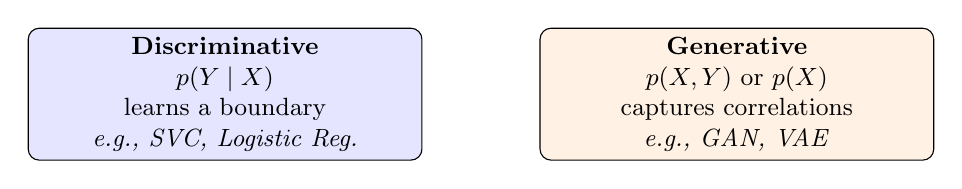
\begin{tikzpicture}[every node/.style={font=\small, align=center}]
    \node[draw, rounded corners, fill=blue!10, minimum width=5cm, minimum height=1.6cm] (disc) at (0,0)
        {\textbf{Discriminative}\\$p(Y \mid X)$\\learns a boundary\\ \emph{e.g., SVC, Logistic Reg.}};
    \node[draw, rounded corners, fill=orange!10, minimum width=5cm, minimum height=1.6cm] (gen) at (6.5,0)
        {\textbf{Generative}\\$p(X, Y)$ or $p(X)$\\captures correlations\\ \emph{e.g., GAN, VAE}};
\end{tikzpicture}
\end{center}

\subsubsection{ Machine Learning: Limitations / Challenges}

This chapter catalogues the fundamental limitations and open challenges of ML models -- a checklist of concerns that must inform the "Robust and Responsible AI" layer of the functional architecture, and that motivates why AI systems require careful engineering beyond just training a model.


\begin{itemize}
    \item \textbf{Opacity, explainability} -- especially for Deep Neural Networks (DNNs), whose internal decision logic is hard to interpret.
    \vspace{0.2cm}
    \item \textbf{Bias (Fairness)} -- models can inherit or amplify biases present in the training data, leading to unfair outcomes for certain groups.
    \vspace{0.2cm}
    \item \textbf{Resource cost} -- computational resources (e.g., for training large models) and human resources (e.g., for data labelling) can be substantial.
    \vspace{0.2cm}
    \item \textbf{Over-/Under-fitting} -- the model may fit training data too closely (overfitting, poor generalization) or too loosely (underfitting, poor performance even on training data).
    \vspace{0.2cm}
    \item \textbf{Vulnerabilities} -- susceptibility to adversarial attacks (linking back to the data-poisoning concern raised in Slide 8).
    \vspace{0.2cm}
    \item \textbf{Bias-Variance Trade-off, Hallucination} -- the classical statistical trade-off between model bias and variance, and (for generative/LLM-based models specifically) the tendency to produce plausible-sounding but factually incorrect output.
    \vspace{0.2cm}
    \item \textbf{"Engineering" challenges} -- storage, processing, distribution, and requirements management (linking back to the entire Data Conditioning discussion of Slides 7--18).
\end{itemize}


\begin{defbox}{Bias-Variance Trade-off}
A model's total prediction error can be decomposed into \emph{bias} (systematic error from overly simplistic assumptions, causing underfitting) and \emph{variance} (sensitivity to fluctuations in the training data, causing overfitting). Reducing one typically increases the other, so model selection requires balancing the two against the specific problem.
\end{defbox}

\begin{defbox}{Hallucination}
A failure mode, particularly prominent in generative models and Large Language Models (LLMs), in which the model produces output that is fluent and plausible in form but factually incorrect or unsupported by the training data/input context.
\end{defbox}

\textbf{Transition.} This chapter closes the purely "Machine Learning" theoretical discussion (Slides 19--21) and sets up the transition to the next macro-topic of the lecture: having established \emph{what} an AI system is made of (functional architecture) and \emph{what} ML methods exist, the lecture now moves to \emph{how} to actually implement, engineer, and manage such a system end-to-end -- the "Implementation Framework".

\subsection{ An End-to-End AI System Architecture Implementation Framework}

This chapter introduces the second major diagram of the course: the \textbf{Implementation Framework}, which answers the \emph{"How"} question (as opposed to the functional architecture of ch 2.1.2, which answered \emph{"What"}). It is adapted from Martinez \& Kifle (2024) and from the AWS Well-Architected Framework.

\begin{defbox}{Implementation Framework}
A structured set of considerations -- organized along \textbf{Technology}, \textbf{Process}, and \textbf{People} dimensions -- that operationalizes the functional architecture blocks (Data Conditioning, ML, Modern Computing, Human-Machine Teaming, Robust/Responsible AI) into a concrete, deployable, and continuously monitored AI product or service.
\end{defbox}

\textbf{Structure of the diagram (left-to-right flow):}

\begin{center}
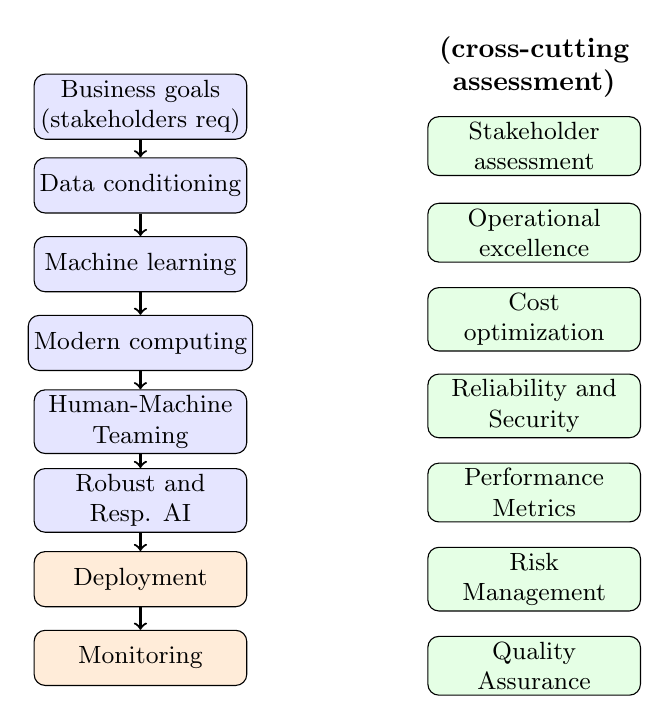
\begin{tikzpicture}[
    every node/.style={font=\small, align=center},
    box/.style={draw, rounded corners, minimum height=0.7cm, minimum width=2.7cm, inner sep=2pt}
]
    % Left column: functional pipeline (from "What")
    \node[box, fill=blue!10] (biz) at (0,5) {Business goals\\(stakeholders req)};
    \node[box, fill=blue!10] (dc) at (0,4) {Data conditioning};
    \node[box, fill=blue!10] (ml) at (0,3) {Machine learning};
    \node[box, fill=blue!10] (comp) at (0,2) {Modern computing};
    \node[box, fill=blue!10] (hmt) at (0,1) {Human-Machine\\Teaming};
    \node[box, fill=blue!10] (rai) at (0,0) {Robust and\\Resp. AI};
    \node[box, fill=orange!15] (dep) at (0,-1) {Deployment};
    \node[box, fill=orange!15] (mon) at (0,-2) {Monitoring};

    \draw[->, thick] (biz) -- (dc);
    \draw[->, thick] (dc) -- (ml);
    \draw[->, thick] (ml) -- (comp);
    \draw[->, thick] (comp) -- (hmt);
    \draw[->, thick] (hmt) -- (rai);
    \draw[->, thick] (rai) -- (dep);
    \draw[->, thick] (dep) -- (mon);

    % Right column: cross-cutting assessment dimensions
    \node[box, fill=green!10] (stake) at (5,4.5) {Stakeholder\\assessment};
    \node[box, fill=green!10] (opex) at (5,3.4) {Operational\\excellence};
    \node[box, fill=green!10] (cost) at (5,2.3) {Cost\\optimization};
    \node[box, fill=green!10] (rel) at (5,1.2) {Reliability and\\Security};
    \node[box, fill=green!10] (perf) at (5,0.1) {Performance\\Metrics};
    \node[box, fill=green!10] (risk) at (5,-1) {Risk\\Management};
    \node[box, fill=green!10] (qa) at (5,-2.1) {Quality\\Assurance};

    \node[font=\bfseries, align=center] at (5,5.5) {(cross-cutting\\assessment)};
\end{tikzpicture}
\end{center}


\pagebreak
\textbf{How to read this diagram.} The left-hand column is essentially the functional-architecture pipeline from Section 2.1.2, now \emph{extended} with two additional stages: \textbf{Deployment} and \textbf{Monitoring} -- making explicit that an AI system's lifecycle does not end once a model is trained, but continues through production release and continuous observation. The right-hand column lists seven \emph{cross-cutting assessment dimensions} that must be applied \emph{at every stage} of the left-hand pipeline, not just once at the end. This is the same "cross-cutting" logic already seen for the "Robust and Responsible AI" layer in Section 2.1.2, now generalized to a full set of engineering/managerial concerns.

\textbf{Framework subtitle: "From input to AI product or service".} This emphasizes that the Implementation Framework's purpose is precisely to bridge the gap between raw input data and a delivered, working AI product/service -- i.e., it is the concrete engineering answer to "How do we build an AI system?" (the question posed back in Slide 3).

\subsubsection{From What to How: Technology}

This chapter details the first of three sub-dimensions of the Implementation Framework: \textbf{Technology}. For each technology-related building block, the slide specifies both a \emph{description} of what must be done and the associated \emph{risk analysis} question.

\begin{center}
\begin{tabular}{p{3cm}p{4.6cm}p{4.6cm}}
\toprule
\textbf{Technology} & \textbf{Description} & \textbf{Risk Analysis} \\
\midrule
System analysis trade-offs & Threshold vs. target requirements, incorporating stakeholders' business goals and the AI capabilities provided. & Can the AI capability be scaled? Are requirements realistic? What is the risk of achieving target vs. threshold requirements? \\[0.2cm]
Functional architecture & The system architecture building block (i.e., the "What" diagram of Slide 6). & End-to-end measure of performance. \\[0.2cm]
Sensors and sources & Identify the data needed. & Are the required data available? \\[0.2cm]
Data condit., ML, computing, HMT & Data preparation; ML algorithm selection; computing (enterprise/edge) infrastructure; addressing the HMT cooperation level. & Technology management and technology levels of maturity. \\[0.2cm]
Robust AI & Vulnerability to adversarial AI. & Likelihood vs. consequence of unintentional/intentional adversaries. \\[0.2cm]
Responsible AI & Use tools to incorporate FASTEPS. & To what degree are harms mitigated and FASTEPS principles implemented? \\
\bottomrule
\end{tabular}
\end{center}

\begin{defbox}{Threshold vs. Target Requirements}
In systems engineering, a \emph{threshold requirement} is the minimum acceptable level of performance for the system to be deemed acceptable, while a \emph{target requirement} is the desired, ideally achieved level of performance. The gap between the two defines the acceptable risk margin during system trade-off analysis.
\end{defbox}

\begin{defbox}{FASTEPS}
An acronym (referenced by the slide as the toolset for implementing "Responsible AI") typically standing for principles such as \textbf{F}airness, \textbf{A}ccountability, \textbf{S}afety, \textbf{T}ransparency, \textbf{E}thics, \textbf{P}rivacy, and \textbf{S}ecurity -- a checklist of responsible-AI dimensions to be actively engineered into the system, not merely aspired to.
\end{defbox}

\textbf{Connection to prior material.} Notice how each row of this table maps directly onto a block of the functional architecture (section 2.1.2): "Sensors and sources" $\rightarrow$ Sensors/Sources block; "Data condit., ML, computing, HMT" $\rightarrow$ the four corresponding functional blocks; "Robust AI" and "Responsible AI" $\rightarrow$ the "Robust and Responsible AI" cross-cutting layer. The Implementation Framework is thus best understood as adding an \emph{engineering discipline layer} (description + risk analysis) on top of each functional block already introduced.

\subsubsection{From What to How: Process (1/2)}

This chapter covers the second dimension of the Implementation Framework: \textbf{Process} (part 1 of 2).

\begin{center}
\begin{tabular}{p{3cm}p{4.6cm}p{4.6cm}}
\toprule
\textbf{Process} & \textbf{Description} & \textbf{Risk Analysis} \\
\midrule
Stakeholder needs & Business goals drive AI requirements. & Are the needs and goals realistic? \\[0.2cm]
Integration, V\&V & Integration, Verification \& Validation (I-V\&V) at each stage of the V-Model (linking back to Slide 4). & Is it exercised at all process levels? \\[0.2cm]
\multicolumn{3}{l}{\emph{(Development, deployment, Monitoring -- flagged as a subsection header on the slide)}} \\[0.1cm]
Operational Excellence & Ability to deliver business value based on the AI value proposition, and to continually improve processes/procedures through monitoring. & Regards all items in "Technology" (Slide 23); must be assessed for each building block. \\[0.2cm]
Cost Optimization & Ability to avoid unneeded costs or suboptimal resource use, throughout the whole system life cycle. & Ability to minimize cost while meeting business needs and goals. \\[0.2cm]
Reliability \& Security & Ability to meet requirements in a secured way. \emph{Reliability}: ability to tolerate/recover from failures and to dynamically acquire resources to meet demand. \emph{Security}: ability to protect information, systems, and assets. Applies to all building blocks. & What is the likelihood of a failure and its associated consequences? \\
\bottomrule
\end{tabular}
\end{center}


\textbf{Reappearance of the V-model.} This slide explicitly reconnects the Implementation Framework to the V-Model of Slide 4: "Integration, V\&V" is precisely the systems-engineering discipline of performing verification/validation \emph{at each stage} of decomposition and integration, not only at the very end.

\subsubsection{ From What to How: Process (2/2)}

Continuation of the Process dimension.

\begin{center}
\begin{tabular}{p{3cm}p{4.6cm}p{4.6cm}}
\toprule
\textbf{Process} & \textbf{Description} & \textbf{Risk Analysis} \\
\midrule
Operational metrics & Performance metrics for each building block, e.g., based on benchmarks (gold standards). Includes accuracy, precision, recall, F-scores, and others relative to model performance and at system-level; also includes efficient use of computing resources and scaling. & (implicitly: whether operational metrics are met at each level) \\[0.2cm]
Risk Management & Includes technical risk (e.g., performance risk), management risk (e.g., cost and schedule), and organizational risk (e.g., societal risk). & Must address the broad range of risks in the context of likelihood vs. consequences (i.e., impact). \\[0.2cm]
Quality Assurance & A broad term to assert that specifications are met (including, e.g., size, weight, power, shock, vibration, ...). Related to the ISO 9000 standard family. & Should be addressed from design to development, deployment, and monitoring; standard compliance. \\[0.2cm]
Cross-cutting system engineering & Tools and approaches to assess performance prior to deployment (e.g., modelling, simulation, emulation, etc.). & Employing these tools should also include the use of operational metrics; these should themselves be checked for quality. \\
\bottomrule
\end{tabular}
\end{center}

\begin{defbox}{Risk Management -- Three Risk Categories}
\begin{itemize}
    \item \textbf{Technical risk} -- e.g., the risk that the system fails to meet performance requirements.
    \item \textbf{Management risk} -- e.g., cost overruns or schedule delays.
    \item \textbf{Organizational risk} -- e.g., broader societal risk arising from the system's deployment.
\end{itemize}
All three must be jointly assessed in terms of \emph{likelihood} $\times$ \emph{consequence (impact)}.
\end{defbox}

\begin{defbox}{ISO 9000}
A family of international standards for \emph{quality management systems}, providing a general framework for ensuring that products/services consistently meet customer and regulatory requirements. Referenced here as the standard family underlying Quality Assurance practices for AI systems.
\end{defbox}

 Note how "Operational metrics" here echoes and quantifies the "System analysis trade-offs" and "End-to-end measure of performance" concerns already raised in the Technology dimension (Slide 23): the Process dimension provides the concrete metrics (accuracy, precision, recall, F-scores, resource efficiency) needed to actually measure whether those Technology-level trade-offs have been achieved.

\subsubsection{From What to How: People}

This  chapter  addresses the third and final dimension of the Implementation Framework: \textbf{People} -- the organizational and human factors required to successfully execute the Technology and Process dimensions covered in Slides 23--25.

\begin{center}
\begin{tabular}{p{3.2cm}p{4.6cm}p{4.4cm}}
\toprule
\textbf{People} & \textbf{Description} & \textbf{Risk Analysis} \\
\midrule
Leadership and management & Leaders define and drive the AI strategic direction and roadmap; managers focus on strategy execution. & Leaders must assess strategic risks; managers address execution risks (e.g., is the necessary talent available to execute a task?). \\[0.2cm]
Systems thinker and systems engineers & Every AI team must include a person with responsibility for and authority over the overall AI system meeting its set of system requirements. & In concert with AI leadership/management, the systems engineer must assess the overall AI system risks. \\[0.2cm]
Staff performance & Management must set clear staff performance goals, and assess progress periodically. & Tools are available (discussed later in the course). \\[0.2cm]
Multicultural environment & AI projects require a multidisciplinary team: engineers, data scientists, ML experts, computing technologists, and human-machine social engineers. & Assess the organization's mentorship and coaching approaches. \\[0.2cm]
Effective communication & Effective communication at all levels within the team and to stakeholders. & This includes ethics issues. \\
\bottomrule
\end{tabular}
\end{center}

\begin{defbox}{The Systems Engineer Role in AI Teams}
A dedicated role, distinct from data scientists or ML engineers, whose responsibility is to hold \emph{overall authority} over whether the AI system as a whole (not just its individual model components) meets the complete set of system-level requirements.
\end{defbox}
